\documentclass[10pt,a4paper]{article}
\usepackage[utf8]{inputenc}

\usepackage{amsmath}
\usepackage{amsfonts}
\usepackage{amssymb}
\usepackage{graphicx}
\usepackage{listings}
\usepackage[margin=1.0in]{geometry}
\usepackage{caption}
\usepackage{subcaption}
\usepackage{float}
\usepackage[utf8]{inputenc}
\usepackage{refstyle}


\lstset{numbers=left,
	title=\lstname,
	numberstyle=\tiny, 
	breaklines=true,
	tabsize=4,
	language=Python,
	morekeywords={with,super,as},,
	frame=single,
	basicstyle=\footnotesize\tt,
	commentstyle=\color{comment},
	keywordstyle=\color{keyword},
	stringstyle=\color{string},
	backgroundcolor=\color{background},
	showstringspaces=false,
	numbers=left,
	numbersep=5pt,
	literate=
		{æ}{{\ae}}1
		{å}{{\aa}}1
		{ø}{{\o}}1
		{Æ}{{\AE}}1
		{Å}{{\AA}}1
		{Ø}{{\O}}1
	}
\usepackage{setspace}
\doublespacing
\usepackage{bm}
\usepackage{hyperref}

\begin{document}

\begin{center}
{\LARGE\bf
FYS4150\\
Project 4, deadline November 15.
}
 
\includegraphics[scale=0.075]{uio.png}\\
Author: Robin D. Kifle,
University of Oslo, Autumn 2017

\vspace{3cm}
{\LARGE\bf
Abstract
}

\end{center}

\newpage

{\LARGE\bf
Introduction
}\\
In this project we will study phase transitions in magnetic systems. We will use the widely popular Ising model in two dimensions.\\
\newpage

{\LARGE\bf
Method
}\\
Before starting on the program we need to find analytical expressions for the partition function Z and the corresponding energy values E, the mean magnetization $|M|$, the specific heat $C_v$ and the susceptibility $\chi$ as functions of the temperature T using periodic boundary conditions.\\
The partition function is given by: $$Z = \sum\limits_{i=1}^{M}e^{-\beta E_i}$$
Where M is the total number of configurations,$\beta$ is the inverse temperature given by $\beta = \frac{1}{kT}$ with k as the Boltzmann constant. $E_i$ is the energy for different spin settings given by: $$E=J\sum\limits_{<kl>}^{N}s_ks_l$$ where J is a constant which expresses the strength of the interaction between spins. N is the total number of configurations.
 $<kl>$ expresses that we only look at the nearest neighbours in the lattice. $s_k$ and $s_l$ are the spins of two neighbouring objects. \\
 For now we work with a 2x2 lattice and the Ising model where the spins can only be in two states, giving a total number of $2^4=16$ configurations.

\begin{center}
\begin{table} [H]
\caption{Energy with periodic boundary conditions and magnetization for different spin-configurations} \label{tab:table5}
\centerline{
\begin{tabular}{c|c|c}
Spin configuration & Energy& Magnetization\\
$\uparrow \uparrow$ &-2J&2\\
$\uparrow \downarrow$&2J&0\\
$\downarrow \uparrow$&2J&0\\
$\downarrow \downarrow$&-2J&-2\\
\end{tabular}
}
\end{table}
\end{center}

From the table above one can observe that the energy is only non-zero on lattices where all objects have the same spin (-8J) and when the diagonals have opposite spin (8J). The magnetization of a 2x2 lattice is only zero when half of the objects have the same spin. We can now calculate the mean energy, the mean absolute magnetization, specific heat and susceptibility with these expressions:\\


Partition function:
$$Z = \sum\limits_{i=1}^{16}e^{-\beta E_i}$$
$$Z = 2e^{8\beta J} + 2e^{-8\beta J}+12$$
$$Z = 4cosh(8\beta J)+12$$

Mean energy:
$$<E> = \frac{1}{Z}\sum\limits_{i=1}^{16}e^{-\beta E_i}E_i$$
$$\sum\limits_{i=1}^{16}e^{-\beta E_i}E_i = -16J(e^{8\beta J}-e^{-8\beta J})=-32Jsinh(8\beta J)$$
$$<E>=-\frac{8J}{cosh(8\beta J)+3}sinh(8\beta J)$$

Mean absolute magnetization:

$$<|M|>=\frac{1}{Z}\sum\limits_{i=1}^{16}e^{-\beta E_i}|M_i|$$
$$\sum\limits_{i=1}^{16}e^{-\beta E_i}|M_i|=8e^{8\beta J}+16$$
$$<|M|>=\frac{2e^{8\beta J}+4}{cosh(8\beta J)+3}$$

Specific heat:
$$C_v = \frac{\beta}{T}(<E^2>-<E>^2)$$
$$<E>^2=\frac{64J^2}{(cosh(8\beta J)+3)^2}sinh^2(8\beta J)$$
\begin{center}
$<E^2>=\frac{1}{Z}\sum\limits_{i=1}^{16}e^{-\beta E_i}E_i^2$ = $\frac{64J^2}{cosh(8\beta J)+3}cosh(8\beta J)$\\
$\rightarrow$
$C_v = \frac{64\beta J^2}{T(cosh(8\beta J)+3)^2}(3cosh(8\beta J)+1)$
\end{center}

Susceptibility:
$$\chi=\beta(<|M|^2>-<|M|>^2)$$
\begin{center}
$<|M|^2>=\frac{1}{Z}\sum\limits_{i=1}^{16}e^{-\beta E_i}M_i^2$ = $\frac{8e^{8\beta J}+8}{cosh(8x)+3}$\\
$\rightarrow$
$\chi = \beta(\frac{8e^{8\beta J}+8}{cosh(8\beta J)+3}-\frac{(2e^{8\beta J}+4)^2}{(cosh(8\beta J)+3)^2})$
\end{center}

Giving these values:

$$<E>=-7.983928$$
$$<|M|>=3.994643$$
$$C_v=0.128329$$
$$\chi=0.016043$$

\noindent Notice that the terms in $C_v$ and $\chi$, $<E^2>-<E>^2$ and $<|M|^2>-<|M|>^2$, respectively, are the variance of the energy and variance of the magnetization.

\newpage

{\LARGE\bf
Method
}\\
uttrykk, algo lagd og funker, 





\newpage

{\LARGE\bf
Results
}\\
After only 10.000 Monte Carlo cycles the numerical solutions for the mean energy and the mean magnetization are close to the values found analytical. They are only off by a value of $10^{-3}$. To get the same magnitude of agreement for the specific heat and susceptibility, 100.000 Monte Carlo cycles was needed. For fewer than 10.000 Monte Carlo cycles the values are irregular.
\begin{center}
\begin{table} [H]
\caption{Analytical and numerical solutions} \label{tab:table1}
\centerline{
\begin{tabular}{c|c|c|c}
& Analytical& Numerical& MC cycles\\
$<E>$&-7.983928&-7.98472& 10.000\\
$<|M|>$&3.994643&3.99494& 10.000\\
$C_v$&0.128329&0.122007& 100.000\\
$\chi$&0.016043&0.015054& 100.000\\
\end{tabular}
}
\end{table}
\end{center}

\begin{figure}[H]
\centerline{
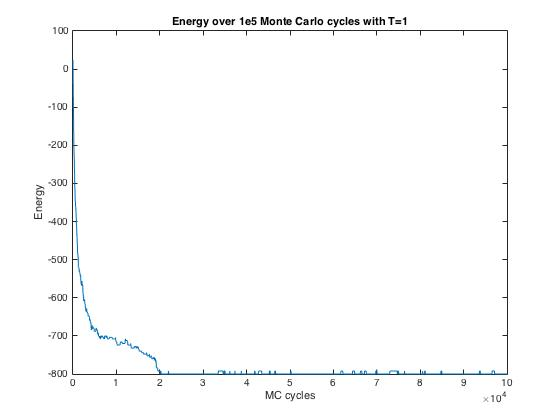
\includegraphics[scale=0.4]{energy20_1e5mc}
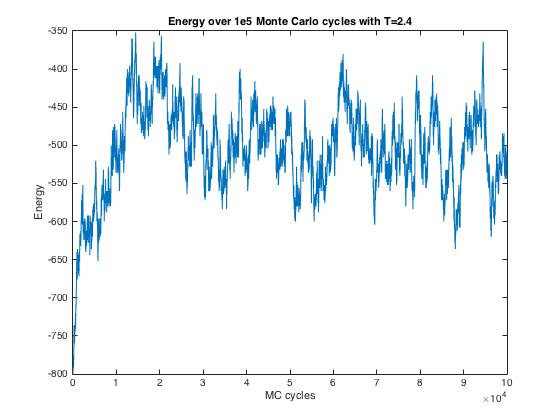
\includegraphics[scale=0.4]{energy20_1e5mc_T24}
}
\caption{Energy vs. Monte Carlo cycles for T=1(left) and T=2.4(right) with random initial 20x20 matrix}
\label{fig:energy_20_1e5}
\end{figure}

\begin{figure}[H]
\centerline{
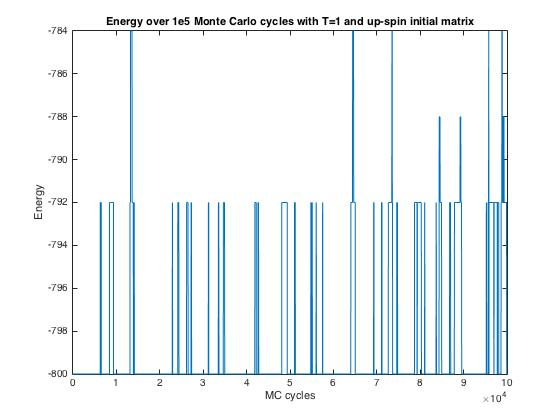
\includegraphics[scale=0.4]{energy20_1e5mc_up}
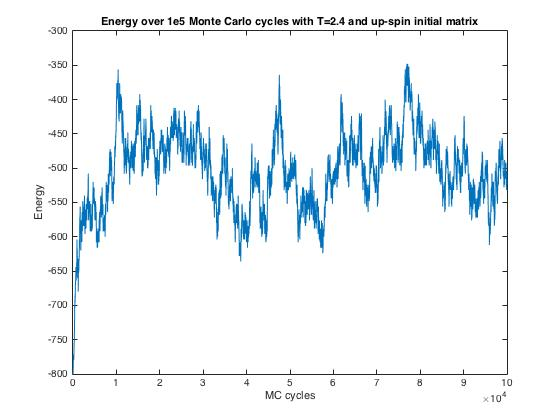
\includegraphics[scale=0.4]{energy20_1e5mc_T24_up}
}
\caption{Energy vs. Monte Carlo cycles for T=1(left) and T=2.4(right) with initial up-spin orientated 20x20 matrix}
\label{fig:energy_20_1e5_up}
\end{figure}

\noindent From \figref{energy_20_1e5} we notice that the random 20x20 lattice with T=1 reach an equilibrium situation after $2*10^4$ Monte Carlo cycles. For T=2.4 the energy oscillates more, but the equilibrium is reached after about the same amount of Monte Carlo cycles. With an initial up-spin oriented matrix the equilibrium is reached more promptly as seen in \figref{energy_20_1e5_up}, after about $7*10^3$ Monte Carlo cycles. The up-spin oriented matrix with a higher temperature oscillates more, but yet again the equilibrium is reached after the same amount of Monte Carlo cycles as for T=1.

\begin{figure}[H]
\centerline{
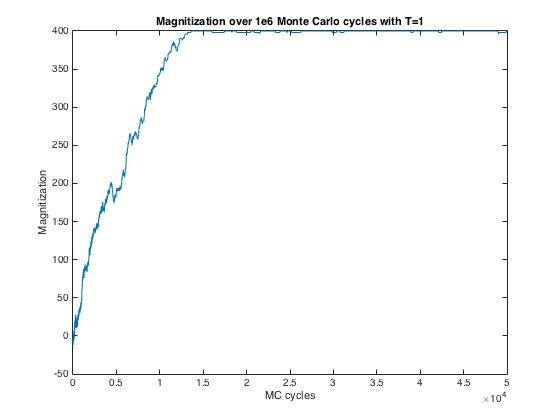
\includegraphics[scale=0.4]{magn20_1e6mc}
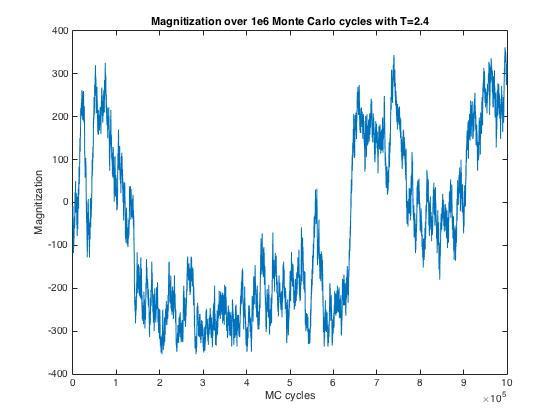
\includegraphics[scale=0.4]{magn20_1e6mc_T24}
}
\caption{Magnitization vs. Monte Carlo cycles for T=1(left) and T=2.4(right) with random initial 20x20 matrix}
\label{fig:magn_20_1e6}
\end{figure}

\begin{figure}[H]
\centerline{
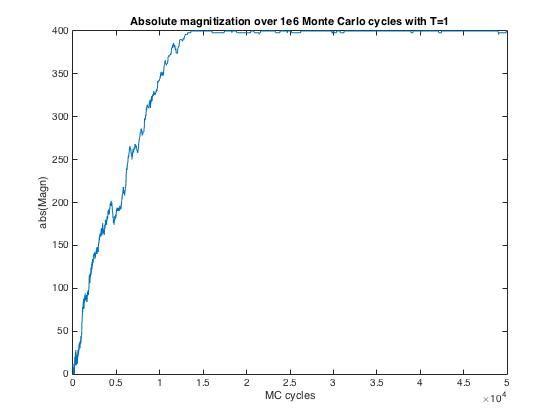
\includegraphics[scale=0.4]{magnAbs20_1e6mc_T=1}
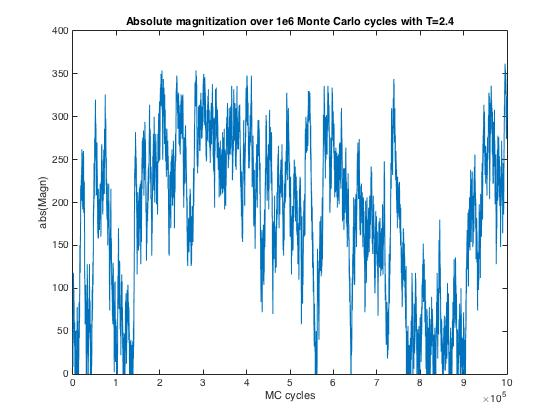
\includegraphics[scale=0.4]{magnAbs20_1e6mc_T=24}
}
\caption{Absolute magnitization vs. Monte Carlo cycles for T=1(left) and T=2.4(right) with random initial 20x20 matrix}
\label{fig:magnAbs_20_1e6}
\end{figure}

\begin{figure}[H]
\centerline{
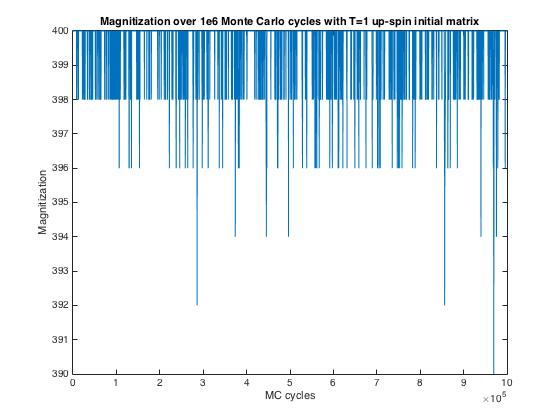
\includegraphics[scale=0.4]{magn20_1e6mc_T=1_up}
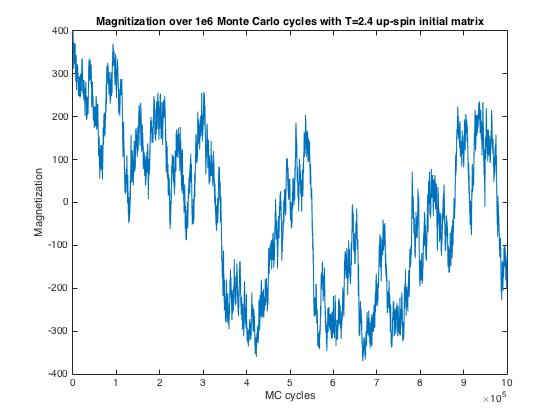
\includegraphics[scale=0.4]{magn20_1e6mc_T24_up}
}
\caption{Magnitization vs. Monte Carlo cycles for T=1(left) and T=2.4(right) with up-spin initial 20x20 matrix}
\label{fig:magn_20_1e6_up}
\end{figure}

\begin{figure}[H]
\centerline{
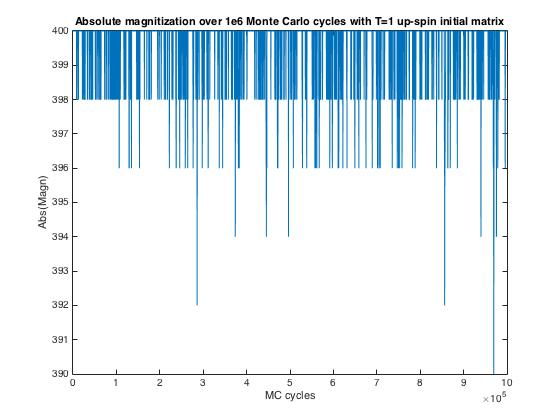
\includegraphics[scale=0.4]{magnAbs20_1e6mc_T=1_up}
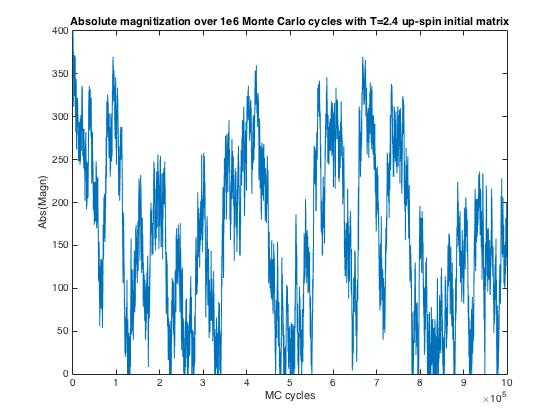
\includegraphics[scale=0.4]{magnAbs20_1e6mc_T24_up}
}
\caption{Absolute magnitization vs. Monte Carlo cycles for T=1(left) and T=2.4(right) with up-spin initial 20x20 matrix}
\label{fig:magnAbs_20_1e6_up}
\end{figure}


\begin{center}
\begin{table} [H]
\caption{Equilibrium values for T=1 T=2.4 for random- and up-spin orientated matrix} \label{tab:table2}
\centerline{
\begin{tabular}{c|c|c|c}
Initial matrix:&Temperature:&Equilibrium&MC cycles\\
Random&1&Random&Random\\
Random&2.4&Random&Random\\
Up-spin&1&400&xx\\
Up-spin&2.4&0 tror jeg&xx\\
\end{tabular}
}
\end{table}
\end{center}

\noindent For a random initial matrix the equilibrium value differs depending on the initial matrix. One of them are shown in \figref{magn_20_1e6}. This one reaches equilibrium after $1.5*10^4$ Monte Carlo cycles with a magnetization value of 400. After multiple runs with different initial matrices they all seem to reach equilibrium before $3*10^4$ Monte Carlo cycles, but the values varies.\\
\\
The up-spin oriented initial matrix with T=1 start with a magnetization equal to its equilibrium value of 400, and does not differ much. Notice the values on the y-axis. When T=2.4 the magnetization oscillates more but blabla

\begin{figure}[H]
\centerline{
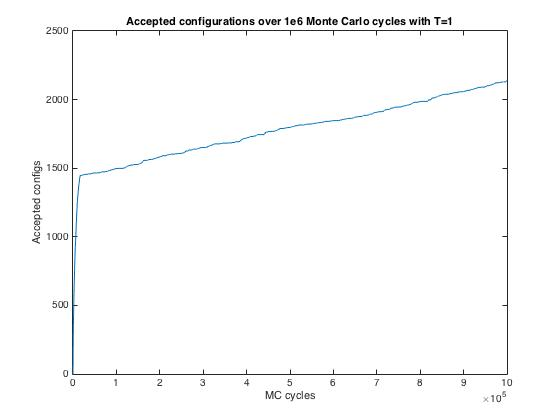
\includegraphics[scale=0.4]{acc20_1e6mc_T=1_ran}
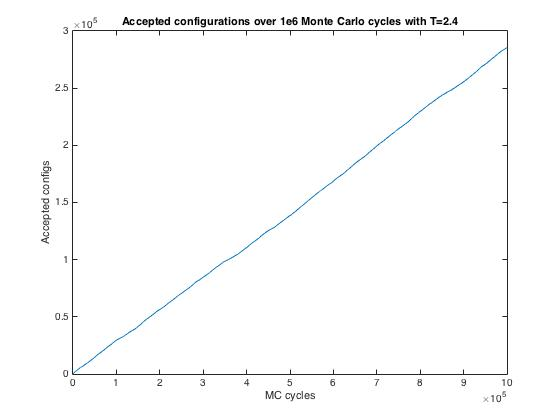
\includegraphics[scale=0.4]{acc20_1e6mc_T=24_ran}
}
\caption{Accepted configurations over $1e^6$ Monte Carlo cycles for T=1(left) and T=2.4(right) for a random initial 20x20 matrix}
\label{fig:configs_20_1e6_rand}
\end{figure}

\begin{figure}[H]
\centerline{
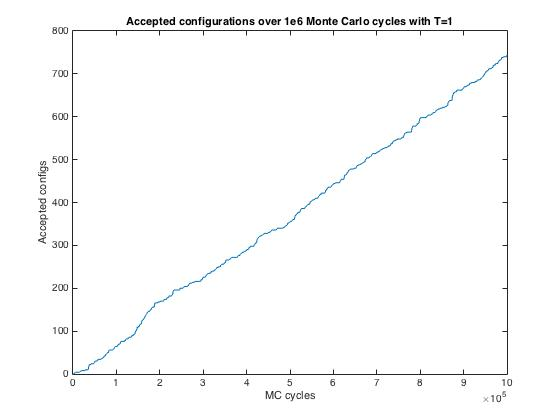
\includegraphics[scale=0.4]{acc20_1e6mc_T=1_up}
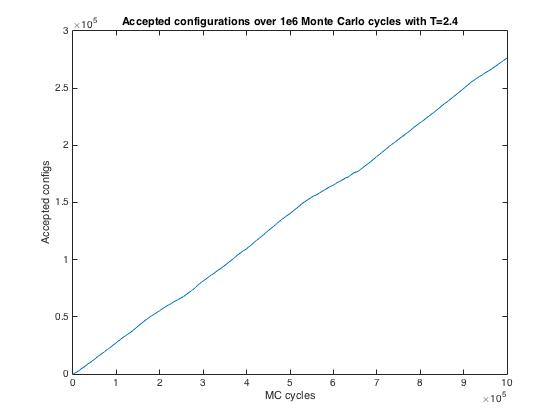
\includegraphics[scale=0.4]{acc20_1e6mc_T=24_up}
}
\caption{Accepted configurations over $1e^6$ Monte Carlo cycles for T=1(left) and T=2.4(right) for a up-spin initial 20x20 matrix}
\label{fig:configs_20_1e6_up}
\end{figure}

\begin{figure}[H]
\centerline{
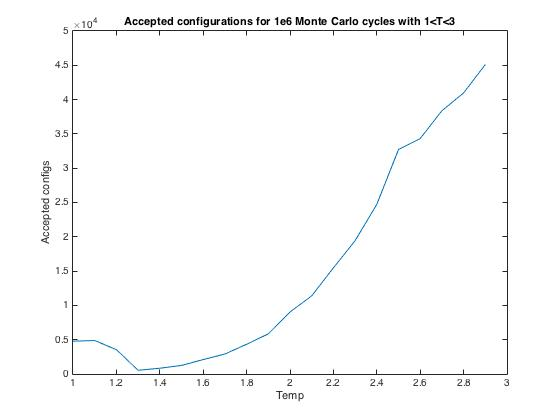
\includegraphics[scale=0.4]{acc20_1T3_1e6_ran}
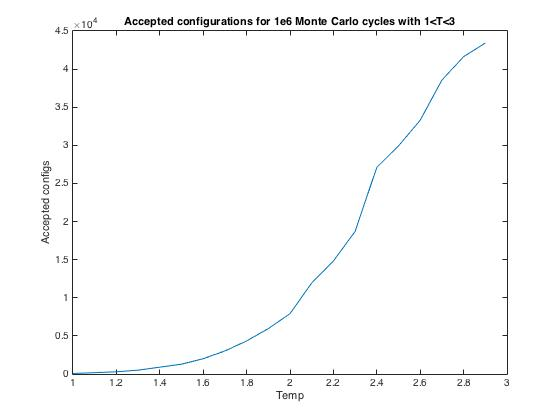
\includegraphics[scale=0.4]{acc20_1T3_1e6_up}
}
\caption{Accepted configurations for $1e^6$ Monte Carlo cycles over $1<T<3$ for a random- and up-spin initial 20x20 matrix, respectively}
\label{fig:configs_T}
\end{figure}

\noindent As seen in \figref{configs_20_1e6_rand}, for a random initial 20x20 matrix and T=1 a lot of configurations are accepted at the start, before quickly (less than $10^5$ Monte Carlo Cycles) reaching an linear state where about the same amount of configurations are accepted. Here it behaves as the initial up-spin matrix seen in \figref{configs_20_1e6_up}. For T=2.4 the random- and up-spin initial matrices behaves the same. They both accept much more configurations and does not seem to reach a state of equilibrium(??).\\
\Figref{configs_T} shows us a exponential growth in accepted configurations for increasing temperatures. There does not seem to be big differences between a random- and a up-spin initial 20x20 matrix.


\newpage
\begin{figure}[H]
\centerline{
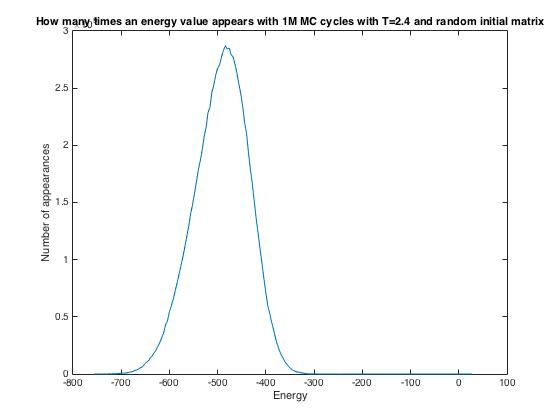
\includegraphics[scale=0.4]{apperances20_1e6_T=24_ran}
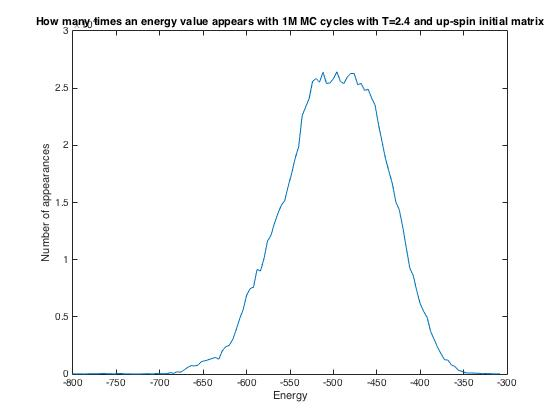
\includegraphics[scale=0.4]{apperances20_1e6_T=24_up}
}
\caption{Probability distribution for T=2.4, random- and up-spin initial 20x20 matrix, respectively}
\label{fig:probdist}
\end{figure}



\begin{center}
\begin{table} [H]
\caption{Variance in energy found graphical and numerical} \label{tab:table3}
\centerline{
\begin{tabular}{c|c|c|c}
Initial matrix:&Temperature:&Variance graphical&Variance numerical(spe heat)\\
Random&1&496.65&496.65\\
Random&2.4&3178.2&3178.24\\
Up-spin&1&9.85&9.85\\
Up-spin&2.4&3151.8&3152.76\\
\end{tabular}
}
\end{table}
\end{center}
graphical in matlab and numerical in c++

\noindent For random- and up-spin initial matrix and T=1 there are almost only the equilibrium value and a small variance. For T=2.4 we notice a negative skewed probability distribution, with the mean value laying on the left side of the mode.

\end{document}